\chapter{Analyse ausgewählter Usability-Probleme}
\section{Situation} \label{sec:analyseSituation}
In einer Liste werden Texte angezeigt, die aus zwei Teilen bestehen. In einem Fall ist der erste Teil ein Schlüssel zur Identifizierung eines Fahrzeuges, der zweite Teil ist der Name des Fahrzeuges. Ein Fahrzeugname kann unter Umständen mehr als einmal auftreten, der Fahrzeugschlüssel hingegen ist eindeutig. Während die Schlüssel sich in der Zeichenanzahl nur um zwei bis drei Zeichen unterscheiden, können die Fahrzeugnamen ganz unterschiedliche Längen haben. Derzeit werden die beiden Textbausteine schlicht aneinandergereiht. Dies führt bei längeren Listen schnell zu Unübersichtlichkeit. Daher sollte eine sichtbare Trennung zwischen den beiden Elementen erfolgen.

\begin{figure}[H]
 \centering
 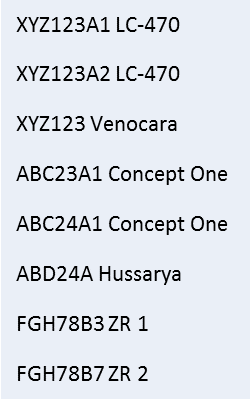
\includegraphics[width=0.3\textwidth]{grafiken/Liste_Beispiel.png}
 \caption{Liste: Ausgangszustand}
 \label{fig:liste1}
\end{figure}

\begin{figure}[H] 
	\centering
	\subfloat[Design 1] {
		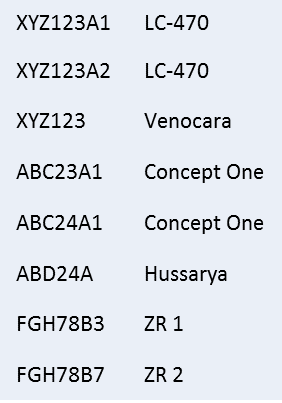
\includegraphics[width=0.3\textwidth]{grafiken/Liste_Design1.png}
	}
	\hspace{1.0em}
	\subfloat[Design 2] {
		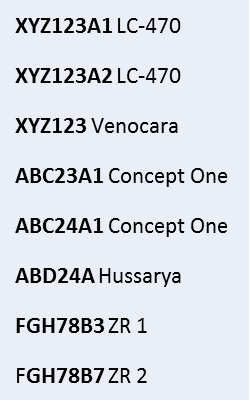
\includegraphics[width=0.265\textwidth]{grafiken/Liste_Design2.png}
	}
	\hspace{1.0em}
	\subfloat[Design 3] {
		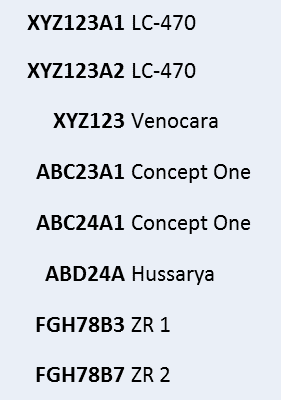
\includegraphics[width=0.3\textwidth]{grafiken/Liste_Design3.png}
	}
	\caption{Design-Vorschläge}
	\label{fig:liste2}
\end{figure}

Alle Design-Vorschläge sind valide Möglichkeiten zur Lösung des Problems, haben jedoch auch ihre Vor- und Nachteile.

Der erste Designvorschlag (Abb. \ref{fig:liste2}(a)) stellt die beiden Teile des Textes sehr gut optisch getrennt dar. Beide Teile sind tabellenartig linksbündig angeordnet. Die ID-Teile aller Texte sind dabei auf einer Höhe, genauso wie die Namensteile. Auf diese Weise entstehen zwei Spalten, in denen die Textbausteine dargestellt werden.

Bei dem zweiten Designvorschlag (Abbildung \ref{fig:liste2}(b)) ist der linke Teil des Textes fett gedruckt, der andere Teil in ganz normalem Stil. Die zweite Lösung setzt zwar die Trennung nicht so sauber wie Vorschlag 1 um, stellt aber so die Fachlichkeit besser dar. Die Fahrzeug ID und der Fahrzeugname sind eine zusammengehörige Einheit. Nach dem Gestaltgesetz der Nähe (Abschnitt \ref{sec:gestaltGesetze}) würden bei Designvorschlag 1 die Fahrzeugschlüssel als eine Objektgruppe und die Fahrzeugnamen als eine Objektgruppe gesehen werden. Da dies nicht die Intention der Abbildung ist, eignet sich die zweite Lösung besser für die Lösung des Problems.

Der dritte Vorschlag gruppiert die Elemente der Liste zwar ebenso wie in Abbildung \ref{fig:liste2}(b), ist jedoch eine eher exotische Darstellungsweise. Hier sind die Elemente an einer gedachten senkrechten Linie zwischen den beiden Teilen angeordnet. Durch die unterschiedliche Bündigkeit entsteht der Eindruck der Gruppierung pro Element, ebenso wie in Vorschlag 2. Durch das Fettdrucken der linken Spalte wird diese dazu hervorgehoben. Das Problem dieser Darstellungsweise ist jedoch der Stilbruch zu den anderen Listendesigns, die im gleichen Bereich angezeigt werden können. Die anderen darstellbaren Listen beinhalten größtenteils keine 2-teiligen Texte. Auf diese Standardvariante der Listen könnte das dritte Design nicht angewandt werden. Es würde daher das Gesetz der Ähnlichkeit (Abschnitt \ref{sec:gestaltGesetze}) verletzt werden und sich so unter Umständen unangenehm auf das Nutzerempfinden auswirken.
\section{Filter-Performance} \label{sec:analyseFilterPerformance}
Die Änderungen, die in Kapitel \ref{sec:implFilter} eingeführt wurden, funktionieren zwar aus technischer Sicht, lassen den Filter aber bei bestimmten Operationen langsam arbeiten, was zu unbequemen Verzögerungen führt.

\textbf{Analyse}

Um die Laufzeitprobleme beheben zu können, mussten als erstes die Fehler gefunden werden, die zu besagten Problemen führten. Bei der Analyse wurden die folgenden Problemfaktoren untersucht:

\begin{itemize}
	\item Zeitintensive Anweisung (möglicherweise in Schleifen ausgeführt?)
	\item Mehrfach hinzugefügte JavaFX-Listener an ObservableLists
	\item Schleifen mit hohen Durchlaufzahlen
	\item Konstruktion von vielen, großen Objekten
\end{itemize}

Für die Überprüfung des ersten Faktors mussten alle Anweisungen einzeln angeschaut werden. Wenn ein Funktionsaufruf dabei ist, der viele Berechnungen ausführt, kann die Ausführungszeit des Aufrufes dadurch gemessen werden, dass der Zeitpunkt vor der Ausführung gespeichert wird und nach der Ausführung von der dann aktuellen Zeit abgezogen wird. Benutzt dafür den Aufruf System\textit{\#currentTimeMillis()} erhält man die Zeitspanne in Millisekunden. Auf diese Weise ließ sich kein performancekritischer Methodenaufruf feststellen. Auch unter Berücksichtigung, dass manche Methoden in Schleifen ausgeführt werden, fand sich keine kritische Stelle.

Die zweite Überprüfung war erfolgreicher. Tatsächlich wurden zwar keine Listener mehrfach an einer ObservableList angehängt, aber pro Werteliste im Filter (in diesem Fall 13) wurden jeweils einige Listener ausgelöst, die diese aktualisieren sollten, wenn sich die ausgewählten Werte geändert haben. Diese Berechnungen erforderten einigen Aufwand und dadurch, dass sie, statt einmal, 13-mal ausgeführt wurden, sorgten sie für eine negative Laufzeitbeeinflussung.

Diese Lösung dieses Problems alleine brachte jedoch nicht den gewünschten Effekt. Eine Methode, die extrem oft ausgeführt wurde und für die meisten Filterberechnungen relevant ist, ist die Methode, die in der Menge der selektierten Werte sucht, ob eine Attribut-Werte-Kombination vorhanden ist.

\begin{lstlisting}[
    language=Java,
    caption=Aufbau - selectedValues,
    label=code12]
	ObservableList<Pair<AbstractFilterAttribute<A>, Object>> selectedValues;
\end{lstlisting}

Als Parameter erhält die Methode ein Attribut und einen Wert, der überprüft werden soll. Die aufgerufene benutzt die \textit{\#contains(Object)}-Methode der List-Implementierung. Dafür muss für jede Überprüfung ein Objekt vom Typ \textit{Pair} erzeugt werden, das das Attribut und den zu überprüfenden Wert kapselt. Zudem muss danach (durch die Implementierung von \textit{\#contains(Object))} jedes Objekt der Liste durchlaufen werden und per \textit{\#equals(Object)} verglichen werden. Je größer die Menge der ausgewählten Werte wird, desto öfter muss ein solcher Vergleich ausgeführt werden. Die Laufzeit eines Durchlaufes über diese Datenstruktur $O(n)$. Bei einzelnen Aufrufen würde dies nicht weiter problematisch werden, doch durch den neuartigen Filter wird diese Methode nun weitaus häufiger ausgeführt.
\section{Quellcode-Usability} \label{sec:quellcodeUsability}
Die Java 8 -Sprachfeatures sind ein gutes Mittel, vor Allem in Kombination mit \gls{javafx} und der \gls{streamAPI}, Code prägnant und sehr kurz darzustellen. Doch haben die neuen Features, vornehmlich Lambdas auch die Eigenschaft, Code schnell zu verkomplizieren, wenn sie im Überfluss verwendet werden. Der durch die Definition bestimmte Nachteil eines \gls{lambda}es ist, dass nicht sofort erkennbar ist, welches Interface implementiert wird und was die Parameter zu bedeuten haben. Dies lässt nicht nur ungeübte Java 8 –Programmierer an einigen Codestellen verzweifeln. Ein Konstrukt, das im Quellcode in einer noch ausgeprägteren Variante zu finden war, wird folgend umrissen.

\begin{lstlisting}[
    language=Java,
    caption=Code-Qualität - Gegenbeispiel,
    label=code13]
	boolen hasSubLevels = level.getListEntries().stream().filter(
			entry -> entry instanceof ILevel).count() > 0;
	entryList.setCellFactory(list -> new ListCell<IListEntry>() { 		//1
		{ setPrefWidth(0); } 																//2
		@Override
		protected void updateItem(IListEntry item, boolean empty) {
			super.updateItem(item, empty);
			[...]
			FalkoArrow arrow = new FalkoArrow(Direction.LEFT);
			arrow.setOpacity(item instanceof ILevel ? 1.0 : 0.0); 			//3
			[...]
			HBox hbox = new HBox(5.0);
			if (hasSubLevels) {
				hbox.getChildren().add(arrow);
			}
			[...]
			setOnMouseClicked((v) -> doCallback(item)); 						//4
			setCursor(empty ? Cursor.DEFAULT : Cursor.HAND);
		}
	});
\end{lstlisting}

Der Code ist zwar sehr knapp aber führt selbst mit Syntax-Coloring schnell zur Unübersichtlichkeit. Dieser Effekt wird dadurch verstärkt, dass das selten verwendete Konstrukt des Instanz-Initializers (2), kombiniert mit einer Anonymen Inneren Klasse als Rückgabewert eines Lambdas eingesetzt wird (1). In dieser Klasse werden zusätzlich ternäre Ausdrücke als Alternative zu If-Klauseln (3) und weitere Lambdas (4) benutzt. Zudem hat die Anonyme Innere Klasse Referenzen in den umschließenden Block (Variable \textit{hasSubLevels}).

Ein weiteres Beispiel hängt mit der Verwendung des Double-Colon-Operators zusammen:

\begin{lstlisting}[
    language=Java,
    caption=Code-Qualität - Gegenbeispiel 2,
    label=code14]
	protected StringProperty specialTextProperty = new SimpleStringProperty("[all values]");
	protected final IListEntry specialEntry = specialTextProperty::get;
\end{lstlisting}

Auch über diesen sehr kurzen Code-Ausschnitt kann sich schnell der Kopf zerbrochen werden. Ein \gls{javafx} StringProperty hat nur die Funktion, einen String-Wert zu kapseln und den Zugriff darauf zu erlauben - über die Funktion \textit{\#get()} und \textit{\#set(String)}. Warum ist der obenstehende Code nicht fehlerhaft? Liefert \textit{\#get()} in diesem Falle doch keinen String zurück?
Es sieht in der Tat für ungeübte Java 8 -Entwickler so aus, als würde der Variable \textit{specialEntry} ein String zugewiesen werden. Doch hier handelt es sich um die Kurzschreibweise eines \gls{lambda}es. Die betroffene Zeile würde wie folgt in einen \enquote{echten} Lambda übersetzt werden:

\begin{lstlisting}[
    language=Java,
    caption=Code-Qualität - Verbesserung,
    label=code15]
	protected final IListEntry specialEntry = () -> specialTextProperty.get();
\end{lstlisting}

Um den Sinn genauer verstehen zu können, muss das Interface IListEntry genauer angeschaut werden. Hier befinden sich zwei Methoden. Eine \gls{defaultImpl} für die Methode \textit{\#getText()} und die abstrakte Methode \textit{\#getValue()}, die die String-Repräsentation von \textit{\#getValue()} zurückliefert. Es muss also die Methode \textit{\#getValue()} des funktionalen Interfaces implementiert werden, damit eine vollständige Klasse entsteht. Genau das machen beide die beiden Code-Ausschnitte \ref{code14} und \ref{code15}. Dennoch ist die Schreibweise zunächst unverständlich.

Dies sind nur zwei Beispiele für schwierig lesbaren Code, im Laufe eines Java 8 -Projektes können viele solcher und ähnlicher Probleme auftreten.